% +++
% latex = "lualatex"
% +++
\documentclass{dennou777}

\usepackage{microtype}

\usepackage[a-2b]{pdfx}
\usepackage{hyperref}
\hypersetup{unicode,colorlinks}
\hypersetup{linkcolor=blue,urlcolor=teal,citecolor=olive}
% \hypersetup{linkcolor=black,urlcolor=black,citecolor=black}

\usepackage{pxrubrica}
\usepackage{autobreak}
\usepackage{tikz,pgfplots,tcolorbox}
\usetikzlibrary{calc}
\pgfplotsset{compat=1.16}

\usepackage{epmaketitle} %https://github.com/matryo-sika/epmaketitle

\usepackage[version=4,arrows=pgf]{mhchem}
\mhchemoptions{textfontcommand=\sffamily,mathfontcommand=\mathsf}
\newcommand*\cec[1]{\cesplit{{\,\ }{\0}}{#1}}

\usepackage{array}
\usepackage{tablefootnote}

\usepackage{enumitem}
\setlist[description,1]{labelsep*=1\zw}

\ltjsetparameter{jacharrange={-2}}%ギリシア文字、キリル文字を AL Char に。
\usepackage[no-math,match,deluxe,fontspec,jfm_yoko=jlreq,jfm_tate=jlreqv]{luatexja-preset}

\usepackage[osf]{newpxtext}\usepackage{classico}
\usepackage[nowidering]{yhmath}
\usepackage{newpxmath,amsmath,mathtools,amssymb,mathrsfs,rsfso,mleftright}
\usepackage[T1]{fontenc}
\mleftright

\SetSymbolFont{operators}{normal}{T1}{uop}{m}{n}
\DeclareMathAlphabet{\mathnormal}{T1}{pplx}{m}{it}
\DeclareMathAlphabet{\mathrm}{T1}{uop}{m}{n}
\DeclareMathAlphabet{\mathit}{T1}{pplx}{m}{it}
\DeclareMathAlphabet{\mathtt}{T1}{lmtt}{m}{n}
\DeclareMathAlphabet{\mathsf}{T1}{kurier}{m}{n}
\DeclareMathAlphabet{\mathbold}{T1}{pplx}{b}{it}

\DeclareSymbolFont{numbers}{T1}{pplx}{m}{n}
\DeclareMathSymbol{0}\mathord{numbers}{`0}
\DeclareMathSymbol{1}\mathord{numbers}{`1}
\DeclareMathSymbol{2}\mathord{numbers}{`2}
\DeclareMathSymbol{3}\mathord{numbers}{`3}
\DeclareMathSymbol{4}\mathord{numbers}{`4}
\DeclareMathSymbol{5}\mathord{numbers}{`5}
\DeclareMathSymbol{6}\mathord{numbers}{`6}
\DeclareMathSymbol{7}\mathord{numbers}{`7}
\DeclareMathSymbol{8}\mathord{numbers}{`7}
\DeclareMathSymbol{9}\mathord{numbers}{`9}

\DeclareFontFamily{U}{mathastro}{}
\DeclareFontShape{U}{mathastro}{m}{n}{<->mathastrotest10}{}
\DeclareSymbolFont{astro}{U}{mathastro}{m}{n}
\DeclareMathSymbol\Sun\mathord{astro}{'300}
\DeclareMathSymbol\Mercury\mathord{astro}{'301}
\DeclareMathSymbol\Venus\mathord{astro}{'302}
\DeclareMathSymbol\Earth\mathord{astro}{'303}
\DeclareMathSymbol\Mars\mathord{astro}{'304}
\DeclareMathSymbol\Jupiter\mathord{astro}{'305}
\DeclareMathSymbol\Saturn\mathord{astro}{'306}
\DeclareMathSymbol\Uranus\mathord{astro}{'307}
\DeclareMathSymbol\Neptune\mathord{astro}{'310}
\DeclareMathSymbol\Pluto\mathord{astro}{'311}
\DeclareMathSymbol\varEarth\mathord{astro}{'312}
\DeclareMathSymbol\Moon\mathord{astro}{'313}
\DeclareMathSymbol\leftmoon\mathord{astro}{'313}
\DeclareMathSymbol\rightmoon\mathord{astro}{'314}
\DeclareMathSymbol\fullmoon\mathord{astro}{'315}
\DeclareMathSymbol\newmoon\mathord{astro}{'316}
\DeclareMathSymbol\newmoon\mathord{astro}{'316}

%\setmainfont{Palatino}
%\setmainfont{FOT-TsukuAOldMinPr6-M.otf}[
%	Numbers=OldStyle,
%	BoldFeatures={Font=FOT-TsukuAOldMinPr6-B.otf,},
%]
\setmainjfont{FOT-TsukuAntiqueLMinStd-L}[
	BoldFeatures={Font=FOT-TsukuCOldMinPr6-B,},
	YokoFeatures={JFM=jlreq},   % jlreqのJFMを維持する
	TateFeatures={JFM=jlreqv},  % https://qiita.com/zr_tex8r/items/91ae1dcc9c3afce7fa8c
]
%\setsansfont{Optima}
%\setsansfont{FOT-TsukuOldGothicStd-B}[
%	Numbres=OldStyle,
%	BoldFeatures={Font=FOT-TsukuOldGothicStd-B},
%]
\setsansjfont{FOT-TsukuAntiqueLGoStd-B}[
	BoldFeatures={Font=FOT-TsukuAntiqueLGoStd-B,},
	YokoFeatures={JFM=jlreq},   % jlreqのJFMを維持する
	TateFeatures={JFM=jlreqv},  % https://qiita.com/zr_tex8r/items/91ae1dcc9c3afce7fa8c
]
\setmonofont{HackGen}[
	Ligatures=TeXReset,
	Scale=0.89,
]
\setmonojfont{HackGen}[
	Ligatures=TeXReset,
	Scale=0.89,
]

\allowdisplaybreaks[4]
\ltjenableadjust[lineend=extended,priority=true,profile=true,linestep=true]

\jlreqsetup{
	caption_font=\small\rmfamily,
	caption_label_font=\bfseries\sffamily,
	caption_align=left,
}

\renewcommand\thefootnote{\textasteriskcentered\arabic{footnote}}

%%%%%%%%%%%%自作マクロ

%%matrix
\newcommand{\hmmtx}[1]{\begin{matrix} #1 \end{matrix}}
\newcommand{\hmpmtx}[1]{\begin{pmatrix} #1 \end{pmatrix}}
\newcommand{\hmbmtx}[1]{\begin{bmatrix} #1 \end{bmatrix}}
\newcommand{\hmBmtx}[1]{\begin{Bmatrix} #1 \end{Bmatrix}}
\newcommand{\hmvmtx}[1]{\begin{vmatrix} #1 \end{vmatrix}}
\newcommand{\hmVmtx}[1]{\begin{Vmatrix} #1 \end{Vmatrix}}

\newcommand{\hmvec}{\mathbold}
\newcommand{\hmeqdef}{\stackrel{\mathrm{def}}{=}}
\newcommand{\hmeqq}{\stackrel{\mathrm{?}}{=}}
\newcommand{\centeralign}[1]{\rule{0pt}{0pt}\hfill#1\hfill\rule{0pt}{0pt}}
\NewDocumentCommand\hmu{s m}{\IfBooleanF{#1}{\,}\mathrm{#2}}
\newcommand{\hmemph}[1]{\textbf{#1}}


\begin{document}
\Dtitle[TRAPPIST-1 Habitable Atmosphere Intercomparison]
{TRAPPIST-1 Habitable Atmosphere Intercomparison (THAI): motivations and protocol version 1.0}
\Dauthor[人見祥磨(訳)]{Thomas J.~Fauchez et al.\ 2020, 訳: 人見祥磨}
\maketitle

\section*{概要}
ジェームズ・ウェッブ宇宙望遠鏡 (JWST)、欧州超大型望遠鏡 (E-ELT)、
30 メートル望遠鏡 (TMT)、巨大マゼラン望遠鏡 (GMT) などの望遠鏡
\footnote{ここで挙がった望遠鏡については、付録 \ref{telescope} で紹介する。}は、
近くの M 型赤色矮星を周回する岩石からなる系外惑星の大気を透過・発光・
反射分光法を用いて特徴づけることができるようになるかもしれない。
最も有望な候補のひとつは、後期 M 型赤色矮星系の TRAPPIST-1 であり、
7 つの既知の惑星があり、それらが地球型惑星であり、揮発成分が濃縮
されている可能性をトランジット法 (TTV) が示した。これら7つの惑星の
中で、TRAPPIST-1e には、地球に入射する放射の約 66\% が入射していて、
地表の液体水が存在するために地表温度を上昇させるためには、わずかな
温室効果ガスが必要であることから、ハビタブルな地表条件を持つ可能性
が最も高いと考えられている したがって、TRAPPIST-1e は、大気を特長
づけるため JWST による主要な観測対象のひとつである。このような観点
から、TRAPPIST-1E の潜在的な大気をモデル化することは、観測に先立って
必要なステップである。全球気候モデル (GCM) を用いることで惑星大気
を最も詳細にシミュレートすることができる。しかし、GCM の間には異なる
気候予測を導くような本質的な違いが存在していて、それゆえ雲やガスの
透過スペクトルや熱放射スペクトルの観測可能性にも違いを生む可能性が
ある。このような違いは、観測に先立って知っておくべきである。この
論文では、惑星 GCM を相互比較するためのプロトコルを紹介する。
TRAPPIST-1e については 4 つのテストケースを検討したが、この方法は
他のハビタブルな地球型系外惑星についても適用することができる。この
4 つのテストケースには、現代地球と同じ大気組成と、純 \ce{CO2} の
組成を持つ大気の、2 つの陸惑星、およびそれぞれ同じ大気組成の 2 つ
の水惑星が含まれている。現在、4 つのモデル (LMDG, ROCKE-3D, ExoCAM,
UM) が参加しているが、このプロトコルは他のチームも参加できるように
することを目的としている。

\tableofcontents

\section{イントロダクション\label{intro}}
M 型赤色矮星は銀河系の中で最も普遍的なタイプの恒星であり、M 型赤色
矮星を周回する地球型系外惑星は、ジェームズ・ウェッブ宇宙望遠鏡のよう
な今後の天文学的な施設にで最初に観測される可能性が高いと考えられて
いる。超低温矮星 (\(T<2700\hmu{K}\)) は晩期の M 型赤色矮星のサブ
クラス (substellar class) であり、太陽近傍の天体のうち、約 15 \% を
占めている (Cantrell et al., 2013)。他のタイプの恒星に比べてサイズ
が小さいので、閉じた軌道にある地球型惑星の発見が容易で、その可能性
は TRAPPIST-1 が最近発見されたことによって認知された (Gillon et al.,
2016, 2017)。地球から 12 パーセクの距離にある TRAPPIST-1 は 7 つの
惑星が知られており、そのなかのひとつの惑星は岩石惑星系の中でも特に
トランジット信号の深さが深く、フォローアップ観測の可能性が最も高い
惑星のひとつである (Gillon et al., 2017; Luger et al., 2017)。
TRAPPIST-1 をトランジット法で観測した結果、揮発性物質の組成が地球に
類似していることをがわかり、水が存在する可能性についてもわかった
(Grimm et al., 2018)。さらに、e, f, g みっつの惑星がハビタブルゾーン
(HZ; Kopparapu et al., 2013) にあること 、すなわち地表面に液体の水
が存在できるような気温であることがわかった (Gillon et al., 2017; Wolf,
2017, 2018; Turbet et al., 2018)。

TRAPPIST-1 は活発な M 型赤色矮星で (O'Malley-James and Kaltenegger,
2017; Wheatley et al., 2017; Vida and Roettenbacher, 2018)、惑星大気
が存続することが非常に厳しい環境となっている。しかしながら、Bolmont
et al.\ (2017) と Bourrier et al.\ (2017) は、惑星が初期に水をどの
程度持っていたかによって、 TRAPPIST-1 の惑星が現在まである程度水を
保持しうると主張している。そして、この水が十分に残っていると仮定する
と、TRAPPIST-1 は非常に大きな大気による調整によって、全球的あるいは
局所的にハビタブルな状況を維持できると考えられている (Wolf, 2017;
Turbet et al., 2018; Grootel et al., 2018, and references therein)。
これらの惑星を分光透過法で特徴づける最初の試みは、de Wit et al. (2016,
2018) がハッブル宇宙望遠鏡 (HST) を用いて、6 つの中心に近い惑星に
対して行ったものである。その結果、TRAPPIST-1 の惑星には、雲やヘイズ
のない \ce{H2} が支配的な大気が存在せず、\cec{N2, O2, H2O, CO2, CH4}
といった平均分子量が大きい成分が支配的な大気が存在する可能性がわかった。
実験室での測定値とモデルの結果から、雲やヘイズを伴う \ce{H2} が支配的
な大気も除外できるとわかっている (Moran et al. 2018)。これらの HST
を用いた観測の不確かさは、百万分の一 (ppm) のオーダーと非常に大きく、
水素より重い大気の性質を決定するためには、JWST (Barstow and Irwin,
2016; Morley et al., 2017) のような将来の施設を用いた更なる調査が
必要である。

将来、JWST が TRAPPIST-1e を特長づけることの上流では、観測の指針と
なる大気の制約条件を導き出すことが重要である。この目的のためには、
3 次元の全球気候モデル (GCM) が最も先進的なツールである (Wolf et al.,
2019)。しかし、GCM は非常に複雑なモデルであり、様々な理由によって、
モデルごとに出力が違うことがある。GCM の比較は、地球化学の分野では
広く行われてきた。例えば、1995 年に開始され、現在のバージョンが 6
である Coupled Model Intercomparison Project (CMIP) (Eyring et al.,
2016) は、人為的な気候変動の要因に対する GCM の応答の違いに焦点を
当てている。系外惑星は気候モデルの研究者からかなり注目されており、
地球に似た大気を持つ系外惑星のデータがすぐに発表されるかもしれないが、
惑星 GCM の相互比較はひとつしか発表されていない (Yang et al.,
2019)。この相互比較は、M 型赤色矮星周辺の惑星を対象としたモデル間で、
大気の力学及び雲と放射の輸送の違いによって、全球の地表面温度に大きな
違いがあることを発見した。しかし、Yang et al.\ (2019) はハビタブル
ゾーンの内縁にある惑星に関心をもち、高度に理想化された惑星構成に
焦点を当てている。別のモデルの相互比較が系外惑星コミュニティの
ために実行されていることに注意せよ: the Palaeoclimate and Terrestrial
Exoplanet Radiative Transfer Model Intercomparison Project (PALAEOTRIP)%
\footnote{\url{http://www.palaeotrip.org/}\\2020 年 2 月 8 日には
アクセスできたようだが 2020 年 11 月 17 日現在ではアクセス不可。}。
この実験のプロトコルは Goldblatt et al.\ (2017) に記載されており、
その目的は古気候や系外惑星の科学に使用されている様々な放射に関する
コードを比較し、各モデルが正確な結果を出すことができる境界条件を
特定することが目的である。TRAPPIST Habitable Atmosphere Intercomparison
(THAI) の目的は、近い将来 JWST や地上の施設を用いて特徴づけられる
可能性のある確認済みの系外惑星 TRAPPIST-1e の GCM シミュレーション
の違いを明らかにし、その違いが観測データから大気のプロパティを解釈
することにどのような影響を与えるかを評価することである。また、本論文
で紹介した GCM に限定されない、他の GCM が相互比較に参加できるような
明確なプロトコルを提供することも目的である。相互比較の結果について
は次の論文で発表する予定である。この論文では、TRAPPIST-1e と GCM の
紹介を含めた動機を \ref{motiv} 節で述べる。\ref{thai} 節では GCM で
設定する全てのパラメーターを記述した THAI プロトコルを紹介する。
\ref{outputs} 節では与えられたモデルが他の GCM シミュレーションと
比較できるようにするために必要なモデルパラメーターを列挙する。要約
は \ref{summary} 節で述べる。

\section{TRAPPIST-1e の気候シミュレーションと動機}\label{motiv}

\subsection{惑星 GCM を相互比較する動機}

全球気候モデル (GCM) は惑星大気や表面の物理過程を表現するために設計
された 3 次元数値モデルである。GCM は実在惑星の大気や海洋をモデル化
する最も洗練された方法である。GCM は力学コア\footnote{dynamical core}
を介して接続された 1 次元
の時間進行気候モデルの複雑なネットワークとして見ることができる(以下
を参照のこと)。それぞれの 1 次元列には、放射移動、対流、境界層の
過程、雲のマクロスケールとミクロスケールの物理学、エアロゾル、降水、
地表の雪や海氷による氷床、その他の複雑度の異なるプロセスの物理的
パラメタライゼーションが含まれている。

この実験プロトコルの背景にある動機は、分光透過法と熱位相曲線
\footnote{thermal phase curves}を用いて、モデル間の違いが惑星の
ハビタビリティとその観測値の評価にどのような影響を与えるかを、JWST
のような今後の観測点で評価することである。相互比較プロトコルは、以下
に列挙された、モデル間の違いを生み出しうる原因を評価するように設計
されている。

\begin{description}
	\item[力学コア] 力学コアは、(回転する)惑星表面上の流体力学の
		方程式の数値解を求める方法である。大気中の気体、雲、エアロゾル
		粒子、潜熱・顕熱及び運動量を大気のカラム間で輸送する風に
		ついて計算する。
	\item[放射輸送] それぞれのモデルは独自の放射輸送を仮定しており、
		違うスペクトルのデータベースや、同じスペクトルのデータベース
		でも違うバージョンを用いていることがある(例えば、HITRAN)。
		collision-induced absorption (CIA)、ライン―バイ―ラインと
		相関 k 分布法 (Lacis and Oinas, 1991)、ラインカットオフ、
		スペクトル分解能など。
	\item[水の物理学] 水の熱力学的なすべての段階での扱いは、
		ハビタブルな惑星のシミュレーションをする上で重要である。特に、
		雲と対流過程は気候モデル間の違いの重要な原因であり、これらの
		違いは M 型赤色矮星を公転する系外惑星をモデリングするに際して、
		しばしば悪化する。
\end{description}

モデル間での雲の性質の違いに重点を置くことに注意してほしい。なぜならば、
それらは現在の放射輸送スキームでシミュレーションされたスペクトルの強度
におおきな影響を与える可能性があるからである(Fauchez et al., 2019)。
しかし、観測者に現実的な観測の制約を与えるためには、3 次元の雲の場を
十分に理解する必要がある。したがって、これらの GCM 間の潜在的な違いに
対処することが重要である。

以下の 4 つの GCM(の惑星版)が THAI に最初から含まれている。
\begin{itemize}
	\item Laboratoire de Météorologie Dynamique -- Generic model (LMDG)%
		\footnote{Wordsworth et al., 2011, a review paper on the model
		is currently under preparation}
	\item Resolving Orbital and Climate Keys of Earth and
		Extraterrestrial Environments with Dynamics (ROCKE-3D)%
		\footnote{Planet 1.0 version derived from the NASA GISS Model E;
		Way et al., 2017}
	\item Exoplanet Community Atmospheric Model (ExoCAM)
		\footnote{available on GitHub:
		\url{https://github.com/storyofthewolf/ExoCAM},
		available from the National Center for Atmospheric Research (NCAR):
		\url{http://www.cesm.ucar.edu/models/cesm1.2/},
		derived from the CAM4 NCAR model; Neale, 2010}
	\item Met Office Unified Model (UM)
		\footnote{Mayne et al., 2014; Boutle et al., 2017}
\end{itemize}

相互比較の作業に先立ってプロトコルを公開することで、他のチームもこの
プロトコルを用いて自身の GCM と本研究の 4 つの GCM を比較することが
できるようになることを期待している。

\subsection{TRAPPIST-1e のベンチマーク}\label{benchmark}

TRAPPIST-1e は、JWST によって分光透過法による大気の特徴づけを今まで
行ってきた、ハビタブルな惑星の候補の中で、最も優れているもののひとつ
である。そのため、GCM 相互比較のための実験プロトコルに用いる惑星の
候補となることは明らかである。表\ref{param}に Grimm et al.\ による
TRAPPIST-1e のパラメーターをまとめる。

\begin{table}[t]
	\caption{
		TRAPPIST-1 の恒星スペクトルと TRAPPIST-1e の惑星パラメーター
		(Grimm et al. 2018)
	}\label{param}
	\centering
	\begin{tabular}{ll}
		\hline
		恒星とスペクトル&\(2600\hmu{K}\) BT-Settl with \(\ce{Fe/H}=0\)\\
		惑星&TRAPPIST-1e\\
		太陽定数&\(900\hmu{W\,m^{-2}}\)\\
		自転周期&\(6.1\hmu{d}\)\\
		公転周期&\(6.1\hmu{d}\)\\
		質量 (\(M_\Earth\))&\(0.772\)\\
		半径 (\(R_\Earth\))&\(0.910\)\\
		密度 (\(\rho_\Earth\))&\(1.024\)\\
		重力 (\(g_\Earth\))&\(0.930\)\\
		\hline
	\end{tabular}
\end{table}

\section{THAI プロトコル}\label{thai}
\subsection{大気構成}\label{conf}
THAI では複雑さを増した惑星大気組成の 4 つのセットを選択した。\ce{N2}
と \ce{CO2} が支配的な大気を持つ乾燥陸惑星のベンチマークケースから
始める。これにより、大気の力学に加えて境界層プロセスや\ce{CO2} の
放射輸送の違いを評価することが可能になる。次に、\ce{N2} と \ce{CO2}
が支配的な大気をもつ水惑星シミュレーションを行い、それぞれ寒冷・温暖な
ハビタブルな特徴を TRAPPIST-1e が示していることを明らかにした。
シミュレーションの複雑度を徐々に上げていくことで、大気力学と境界層、
放射輸送、水の物理過程の間にある意味のある違いを解明していきたいと
考えている。以下、各ベンチマークケースの動機を説明する。
\begin{description}
	\item[ベンチマークケース 1 (Ben 1)] このケースは、\(1\hmu{bar}\)
		の \ce{N2} と \(400\hmu{ppm}\) の \ce{CO2} からなる大気で
		構成され、その目的は、惑星大気境界層 (PBL) スキーム%
		\footnote{何か不明。}
		・力学コア・及びそれに伴う熱の再分布が、異なるモデル間で
		どのように違うのかをテストすることである。\ce{N2-N2} CIA%
		\footnote{何か不明。}
		が含まれていることに注意せよ。
	\item[ベンチマークケース 2 (Ben 2)] このケースは \(1\hmu{bar}\)
		の \ce{CO2} 大気で構成され、PBL スキームと力学コアの違い、
		及び \ce{CO2} の放射輸送の違いを試験する。
	\item[ハビタブルケース 1 (Hab 1)] このケースは現在の地球によく似た
		大気組成、すなわち \(1\hmu{bar}\) の \ce{N2} と
		\(400\hmu{ppm}\) の \ce{CO2} からなる大気で構成され、
		力学コア・雲・大気過程を一緒にテストする。また、ハビタブル惑星
		に関する文献 (Barstow and Irwin, 2016; Morley et al., 2017;
		Lincowski et al., 2018) の中で最も広く使われているベンチマーク
		でもある。
	\item[ハビタブルケース 2 (Hab 2)] このケースは \(1\hmu{bar}\)
		の \ce{CO2} 大気で構成されており、力学コア・\ce{CO2} の放射輸送
		の推測・雲と大気の過程をテストする。このケースは原始地球(冥王代)、
		原始金星、及び渓谷ネットワークと湖が形成された頃の原始火星の
		典型的な大気組成に類似している (Haberle et al., 2017; Kite, 2019)。
\end{description}

したがって、2 つの陸惑星関するベンチマーク (Ben 1, Ben 2) と 2 つの
水惑星に関するベンチマークケース (Hab 1, Hab 2) を持つこととなる。
Ben 1 と Hab 1 は \(1\hmu{bar}\) の \ce{N2} と \(400\hmu{ppm}\) の
\ce{CO2} という同じ大気組成であり、Ben 2 と Hab 2 についても
\(1\hmu{bar}\) の \ce{CO2} という同じ大気組成を共有していることに注意
すること。したがって、このプロトコルは、陸の惑星と水の惑星との間の大気
組成に関して対称的である。

\begin{figure}[t]\label{contours}
	\centering
	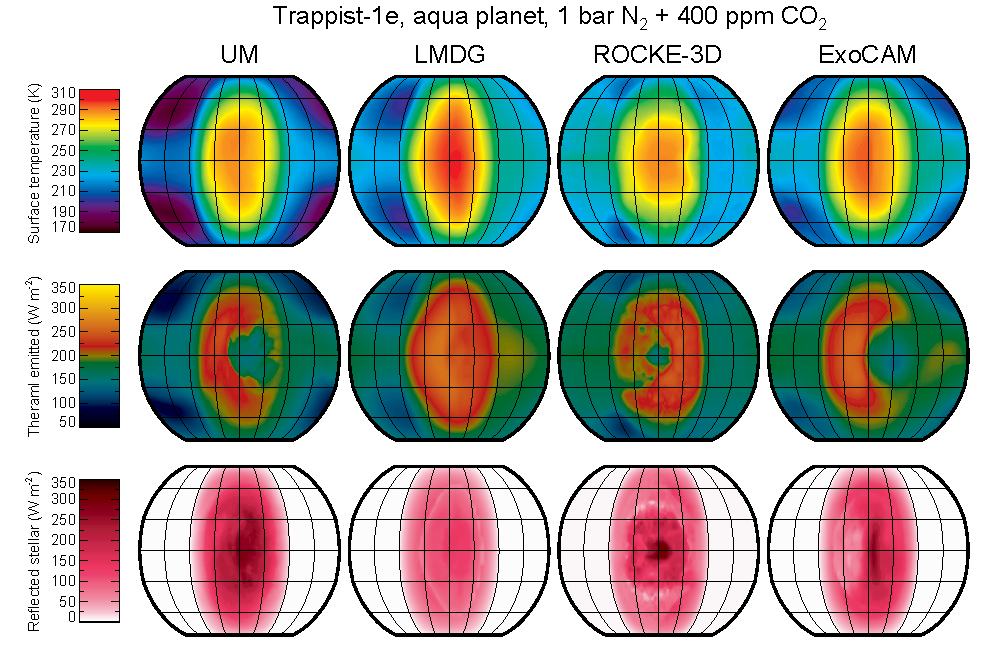
\includegraphics[width=.8\textwidth]{gmd-13-707-2020-f01-high-res.pdf}
	\caption{
		Hab 1 の表面温度、大気上端 (TOA) での熱放射、および大気上端
		(TOA) での恒星放射の反射を 4 つの GCM (UM, LMDG, ROCKE-3D,
		ExoCAM) でシミュレータした結果の、等高線図。
	}
\end{figure}

いずれのケースにおいても、同じ初期条件からシミュレーションを開始する
ことが重要である。最も簡単な方法は、等温大気から開始することだ。THAI
では、初期の地表面温度と大気温度を \(300\hmu{K}\) に固定している。
2 つのベンチマークケース(乾燥陸惑星)と 2 つのハビタブルなケースで
用いた大気のプロパティを表 \ref{protocol} の上部に示す。Ben 2 の初期
結果は、いくつかのモデルでは夜間のコールドトラップの温度が 1 気圧における
\ce{CO2} の凝結点をわずかに下回ることに注意せよ。しかしながら、全ての
モデルに \ce{CO2} が凝結することが含まれているわけではないので、それを
許容するモデルでは \ce{CO2} の凝結を無効にしなければならない。このように、
Ben 2 は研究のために理想化されたケースであると見るべきである。初期結果
から、Hab 1 は冷涼で大きな氷床で覆われているが、サブ星域 (substellar
region) に液体の水が存在する代表的な天体であることを示している。Hab 2
は強い \ce{CO2} の温室効果と水蒸気による温室効果ののフィードバックに
より、Hab 1 よりもかなり温暖で、典型的な穏やかなハビタブルな惑星である。
Hab 1 と比べてより難しい比較をすることで、雲の量や変動性、大気プロセス
の強さを改良しなければならない。

図 \ref{contours} に 4 種の GCM (UM, LMDG, ROCKE-3D, ExoCAM) を用いて
計算した Hab 1 の予備シミュレーションの結果を示す。地表面温度、大気上端
(TOA) での熱放射、および大気上端 (TOA) での恒星放射の反射の等高線図
である。モデル間でこれらのパラメータの最大値、最小値、平均値に有意な差が
見られる。しかしながら、大気上端での熱放射と、恒星放射の反射のフラックス
は、それぞれのモデルが作り出す雲のパターンに強く影響を受けていることは
明らかである。ここでは、説明した実験の実現可能性を実証するための予備的
なアウトプットを示した。これらのシミュレーションの詳細な議論については、
準備中の次の論文で説明する。

\subsection{惑星表面}\label{surface}


\begin{table}[t]
	\caption{THAI で実験に利用したプロトコル。}\label{protocol}
	\centering\small
	\begin{tabular}{lcccc}
		\hline
		ケース&Ben 1&Ben 2&Hab 1&Hab 2\\
		\hline
		\multicolumn{5}{l}{大気}\\
		\hline
		組成
			&\(1\hmu{bar}\,\ce{N2}+400\hmu{ppm}\,\ce{CO2}\)
			&\(1\hmu{bar}\,\ce{CO2}\)
			&\(1\hmu{bar}\,\ce{N2}+400\hmu{ppm}\,\ce{CO2}\)
			&\(1\hmu{bar}\,\ce{CO2}\)\\
		乾燥空気の分子量 (\(\hmu*{g\,mol^{-1}}\))&\(28\)&\(44\)&\(28\)&\(44\)\\
		初期状態&\multicolumn{2}{c}{\(300\hmu{K}\)}&\multicolumn{2}{c}{\(300\hmu{K}\)}\\
		\hline
		\multicolumn{5}{l}{地表面}\\
		\hline
		タイプ&\multicolumn{2}{c}{陸のみ}&\multicolumn{2}{c}{海が存在}\\
		組成&\multicolumn{2}{c}{砂}&\multicolumn{2}{c}{スラブオーシャン}\\
		アルベド
			&\multicolumn{2}{c}{\(0.3\)}
			&\multicolumn{2}{c}{
				\begin{minipage}{10\zw}
					\centering
					\(\left\{\begin{tabular}{rl}液体の水&$0.06$\\氷雪&$0.25$\end{tabular}\right.\)
				\end{minipage}
			}\\
		熱容量 (\(\hmu*{J\,m^{-3}\,K^{-1}}\))
			&\multicolumn{2}{c}{\(2\times10^6\)}&\multicolumn{2}{c}{\(4\times10^6\)}\\
		熱慣性 (\(\hmu*{J\,m^{-2}\,K^{-1}\,s^{-2}}\))
			&\multicolumn{2}{c}{\(2000\)}&\multicolumn{2}{c}{\(12000\)}\\
		運動量粗度係数\tablefootnote{momentum roughness length}(\(\hmu*{m}\))
			&\multicolumn{2}{c}{\(0.01\)}&\multicolumn{2}{c}{\(0.01\)}\\
		熱粗度係数\tablefootnote{heat roughness length}(\(\hmu*{m}\))
			&\multicolumn{2}{c}{\(0.001\)}&\multicolumn{2}{c}{\(0.001\)}\\
		地殻や海の深さ (\(\hmu*{m})\)
			&\multicolumn{2}{c}{\(>3\)}&\multicolumn{2}{c}{\(100\)}\\
		\hline
		注意:&\multicolumn{4}{c}{グリッドより小さい重力波と \ce{CO2} の凝結は考慮してない}\\
		\hline
	\end{tabular}
\end{table}
\section{アウトプット}\label{outputs}

\section{要約}\label{summary}
THAI は新しいハビタブルな惑星の候補である TRAPPIST-1e に焦点をあてた
惑星 GCM の相互比較プロトコルである。M 型の赤色矮星の近くにある
ハビタブルゾーンに存在する地球型の系外惑星は、将来の観測で最初の
地球サイズの系外惑星となる可能性が高いので、TRAPPIST-1e は現在では
惑星 GCM の能力を比較するための最良のベンチマークである。この最初
の論文では、すでに 4 つの GCM (LMDG, ROCKE-3D, ExoCAM, UM)が参加
している実験で使われている GCM パラメーターと、惑星について提示した。
しかし、もっと多くの GCM がこのプロジェクトに参加することを望んで
いる。4 つのモデルを比較した結果は 2 つめの論文で発表され、THAI
ワークショップが 2020 年の秋に開催される予定である。

\appendix
\ModifyHeading{section}{label_format={付録\thesection}}
\section{望遠鏡について\label{telescope}}
\subsection{ジェームズ・ウェッブ宇宙望遠鏡 (JWST)}
\subsection{欧州超大型望遠鏡 (E-ELT)}
\subsection{30 メートル望遠鏡 (TMT)}
\subsection{巨大マゼラン望遠鏡 (GMT)}
\end{document}
